\documentclass{beamer}
\usetheme{CambridgeUS}
\setbeamertemplate{footline}[frame number] % Affiche uniquement le numéro de page
\usepackage[utf8]{inputenc}
\usepackage{graphicx}
\usepackage{hyperref}

\title{Edge Computing: A Decentralized Evolution of the Cloud}
\author{Galiléa LE MOULLEC (Mun ID: 202415993) \and Félicien MOQUET (Mun ID: 202415994)}
\institute{Memorial University of Newfoundland, St. John's, Canada}
\date{March 2025}

\begin{document}

\begin{frame}
  \titlepage
\end{frame}

%--- Slide 1: Introduction ---
\begin{frame}{Introduction}
  \begin{itemize}
    \item Rapid growth of connected devices and real-time applications
    \item Traditional cloud computing reaches its limits
    \item \textbf{Edge computing} brings computation closer to the data source
  \end{itemize}
\end{frame}

%--- Slide 2: Why Edge Computing? ---
\begin{frame}{Why Edge Computing?}
  \begin{itemize}
    \item \textbf{Latency:} Reduces delay for real-time responses
    \item \textbf{Bandwidth:} Minimizes data transfer volume
    \item \textbf{Privacy:} Keeps sensitive data local
    \item \textbf{Resilience:} Operates even with cloud disconnections
  \end{itemize}
\end{frame}

%--- Slide 3: Architecture Overview ---
\begin{frame}{Architecture Overview}
  \begin{itemize}
    \item \textbf{Edge devices:} Sensors, wearables, cameras
    \item \textbf{Edge nodes:} Gateways, micro-servers, local processors
    \item \textbf{Cloud layer:} For large-scale analytics and storage
  \end{itemize}
  \vspace{0.5cm}
  \centering
  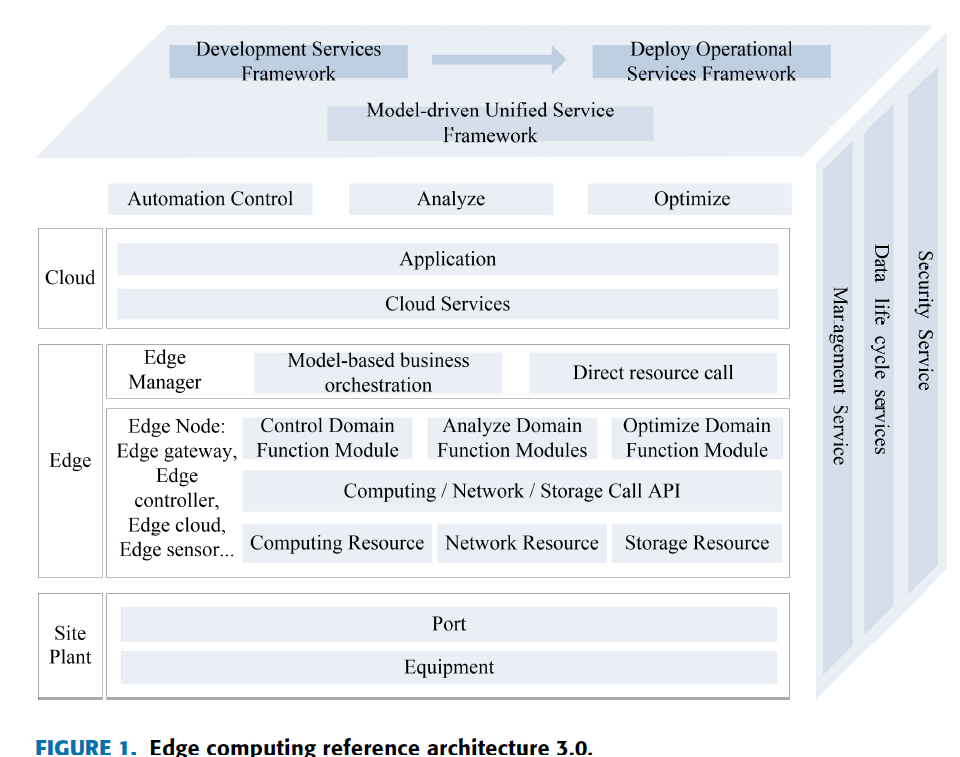
\includegraphics[width=0.6\linewidth]{IMG/6.png} % Optional
\end{frame}

%--- Slide 4: Use Case - IoT ---
\begin{frame}{Use Case: Internet of Things (IoT)}
  \begin{itemize}
    \item Smart homes: temperature, lighting, security
    \item Environmental monitoring: air quality, agriculture
    \item Local processing improves responsiveness and privacy
  \end{itemize}
\end{frame}

%--- Slide 5: Use Case - Autonomous Vehicles ---
\begin{frame}{Use Case: Autonomous Vehicles}
  \begin{itemize}
    \item Onboard sensors generate huge data streams
    \item Requires instant decision-making (e.g. braking)
    \item Edge computing enables safety-critical operations
  \end{itemize}
\end{frame}

%--- Slide 6: Use Case - Smart Cities ---
\begin{frame}{Use Case: Smart Cities}
  \begin{itemize}
    \item Real-time traffic management
    \item Public safety and surveillance
    \item Energy optimization and environmental monitoring
  \end{itemize}
\end{frame}

%--- Slide 7: Use Case - Healthcare ---
\begin{frame}{Use Case: Healthcare and Telemedicine}
  \begin{itemize}
    \item Real-time patient monitoring
    \item On-site diagnostics in emergencies
    \item Strong data privacy and compliance (e.g. GDPR)
  \end{itemize}
\end{frame}

%--- Slide 8: Pros and Cons ---
\begin{frame}{Advantages and Challenges}
  \textbf{Advantages:}
  \begin{itemize}
    \item Lower latency and bandwidth usage
    \item Better data privacy and security
    \item Improved resilience and scalability
  \end{itemize}
  \vspace{0.3cm}
  \textbf{Challenges:}
  \begin{itemize}
    \item Complex management of distributed nodes
    \item Interoperability with cloud platforms
    \item Security at the edge
  \end{itemize}
\end{frame}

%--- Slide 9: Trends and Future Perspectives ---
\begin{frame}{Trends and Future Perspectives}
  \begin{itemize}
    \item Integration with AI and 5G for smarter edge decisions
    \item Lightweight containers and orchestration (e.g. K3s)
    \item Research in privacy-preserving analytics, federated learning
  \end{itemize}
\end{frame}

%--- Slide 10: Conclusion ---
\begin{frame}{Conclusion}
    \begin{itemize}
      \item Edge computing addresses key limitations of centralized cloud
      \item Use cases show strong benefits in latency, privacy, and efficiency
      \item Future: a hybrid cloud-edge ecosystem
    \end{itemize}
    \vspace{0.3cm}
    Thank you!\\
  \end{frame}

%--- Slide 11: Open Question / Discussion ---
\begin{frame}{Open Discussion}
  \begin{block}{\textbf{Discussion Point}}
    Edge computing reduces data exchanges by processing locally. But:\\
    \textbf{With network demands constantly rising, will edge computing be enough?}\\
    Or is it just a temporary relief before a new saturation point?
  \end{block}
\end{frame}



\end{document}